\subsection{Determinism}

\begin{frame}{What Markov categories are \emph{not}}
	\begin{definition}
		A symmetric monoidal category with 
		\begin{itemize}
			\item objects: commutative comonoids $(X, \del_X, \cop_X)$ 
			\item morphisms: morphisms of comonoids
		\end{itemize}
	\end{definition}
	\pause
	$f : X \to Y$ preserves comultiplication iff
%	\[\tikzfig{deterministic}\]
	\begin{center}
	\begin{tabular}{ccc}
		\tikzfig{deterministic_l} 
		& $=$
		& \tikzfig{deterministic_r}
		\\ \\ \pause
		run $f$ twice 
		&& run $f$ once\\
		with same input
		&& and copy output
	\end{tabular}
	\end{center}
\end{frame}

%TODO: strikeout

%\begin{frame}{Copy and Delete}
%	In Markov category: 
%	morphism $f : X \to Y$ in general \textit{not} morphisms of comonoids $(X, \del_X, \cop_X) \to (Y, \del_Y, \cop_Y)$: 
%%	\begin{itemize}
%%		\item 
%%		$I \in \cC_0$ is \textit{terminal}\\
%%		$\Leftrightarrow$ 
%%		morphisms 
%%		%$\Leftrightarrow$
%%		%$(\del_X : X \to I)_{X}$ is natural in $X \in \cC_0$.\\
%%		Interpretation: randomness is \textit{normalized}
%%		\item 
%%		copying does (in general) not preserve comonoid structure\\
%%		%$\Leftrightarrow$
%%		%$(\cop_X : X \to X \otimes X)_{X}$ is \textit{not} natural.\\
%%		Interpretation: ?
%%	\end{itemize}
%\begin{tabular}{c c}
%		\multicolumn{2}{l}{$f$ preserves counits:}\\
%		\begin{tikzcd}[ampersand replacement=\&]
%		X \& \& Y \\
%		\& I
%		\arrow[""{name=0, anchor=center, inner sep=0}, "f", from=1-1, to=1-3]
%		\arrow["{\del_X}"', from=1-1, to=2-2]
%		\arrow["{\del_Y}", from=1-3, to=2-2]
%		\arrow["\scalebox{1.5}{$\circlearrowleft$}"{description}, draw=none, from=0, to=2-2]
%		\end{tikzcd}
%		&	\tikzfig{counitality}
%		\\
%		\multicolumn{2}{l}{Interpretation: \textit{normalized} randomness} 
%		\\
%		\multicolumn{2}{l}{$f$ does \textit{not} preserve comultiplication:}\\
%		\begin{tikzcd}[ampersand replacement=\&]
%			X \&\& Y \\
%			\\
%			{X \otimes X} \&\& {Y \otimes Y}
%			\arrow[""{name=0, anchor=center, inner sep=0}, "f", from=1-1, to=1-3]
%			\arrow["{\cop_X}"', from=1-1, to=3-1]
%			\arrow["{\cop_Y}", from=1-3, to=3-3]
%			\arrow[""{name=1, anchor=center, inner sep=0}, "{f \otimes f}"', from=3-1, to=3-3]
%			\arrow["\scalebox{1.5}{$\bcancel{\circlearrowleft}$}"{description}, draw=none, from=0, to=1]
%		\end{tikzcd}
%		&	\tikzfig{non-deterministic}		
%		\\ 
%		\multicolumn{2}{l}{Interpretation: $f$ \textit{has randomness}}
%\end{tabular}
%\end{frame}

%\begin{frame}{Determinism}
%	A $f$ process with \emph{uncertainty} does \emph{not} preserve comultiplication:\\
%		\begin{tabular}{ccc}
%			\tikzfig{deterministic_l} 
%			& $\neq$
%			& \tikzfig{deterministic_r}
%			\\
%			run $f$ multiple times 
%			&& run $f$ once\\
%			with same input
%			&& and copy output
%		\end{tabular}
%\end{frame}

\begin{frame}{Determinism in Markov categories}
\begin{definition}
	$f : X \to Y$ is \emph{deterministic} if
	\begin{equation*}
		\tikzfig{deterministic}
	\end{equation*}
\end{definition}
%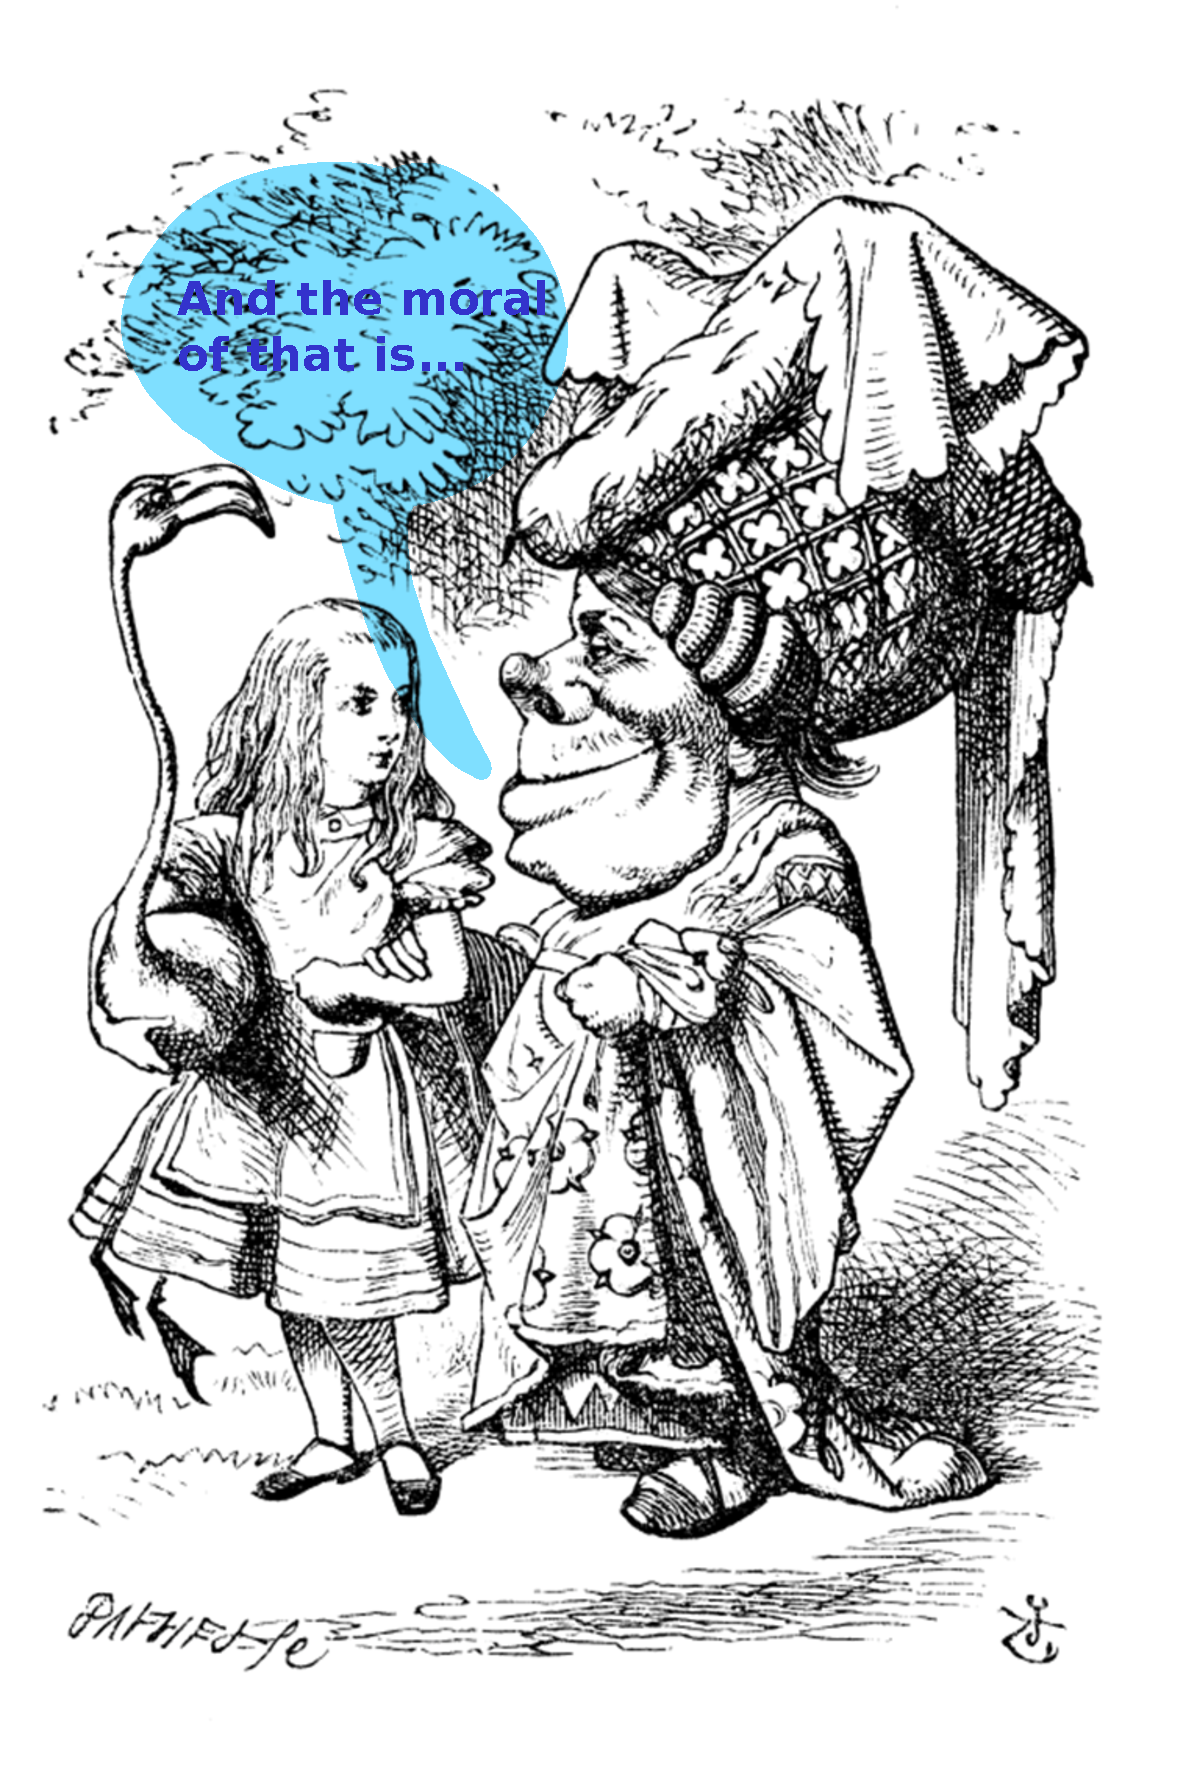
\includegraphics[scale=0.3]{part2/Figures/1-the-duchess-moral}
\end{frame}

%\begin{frame}{Determinism}
%	\begin{minipage}{0.4\linewidth}
%		\begin{center}
%			\makebox[\textwidth]{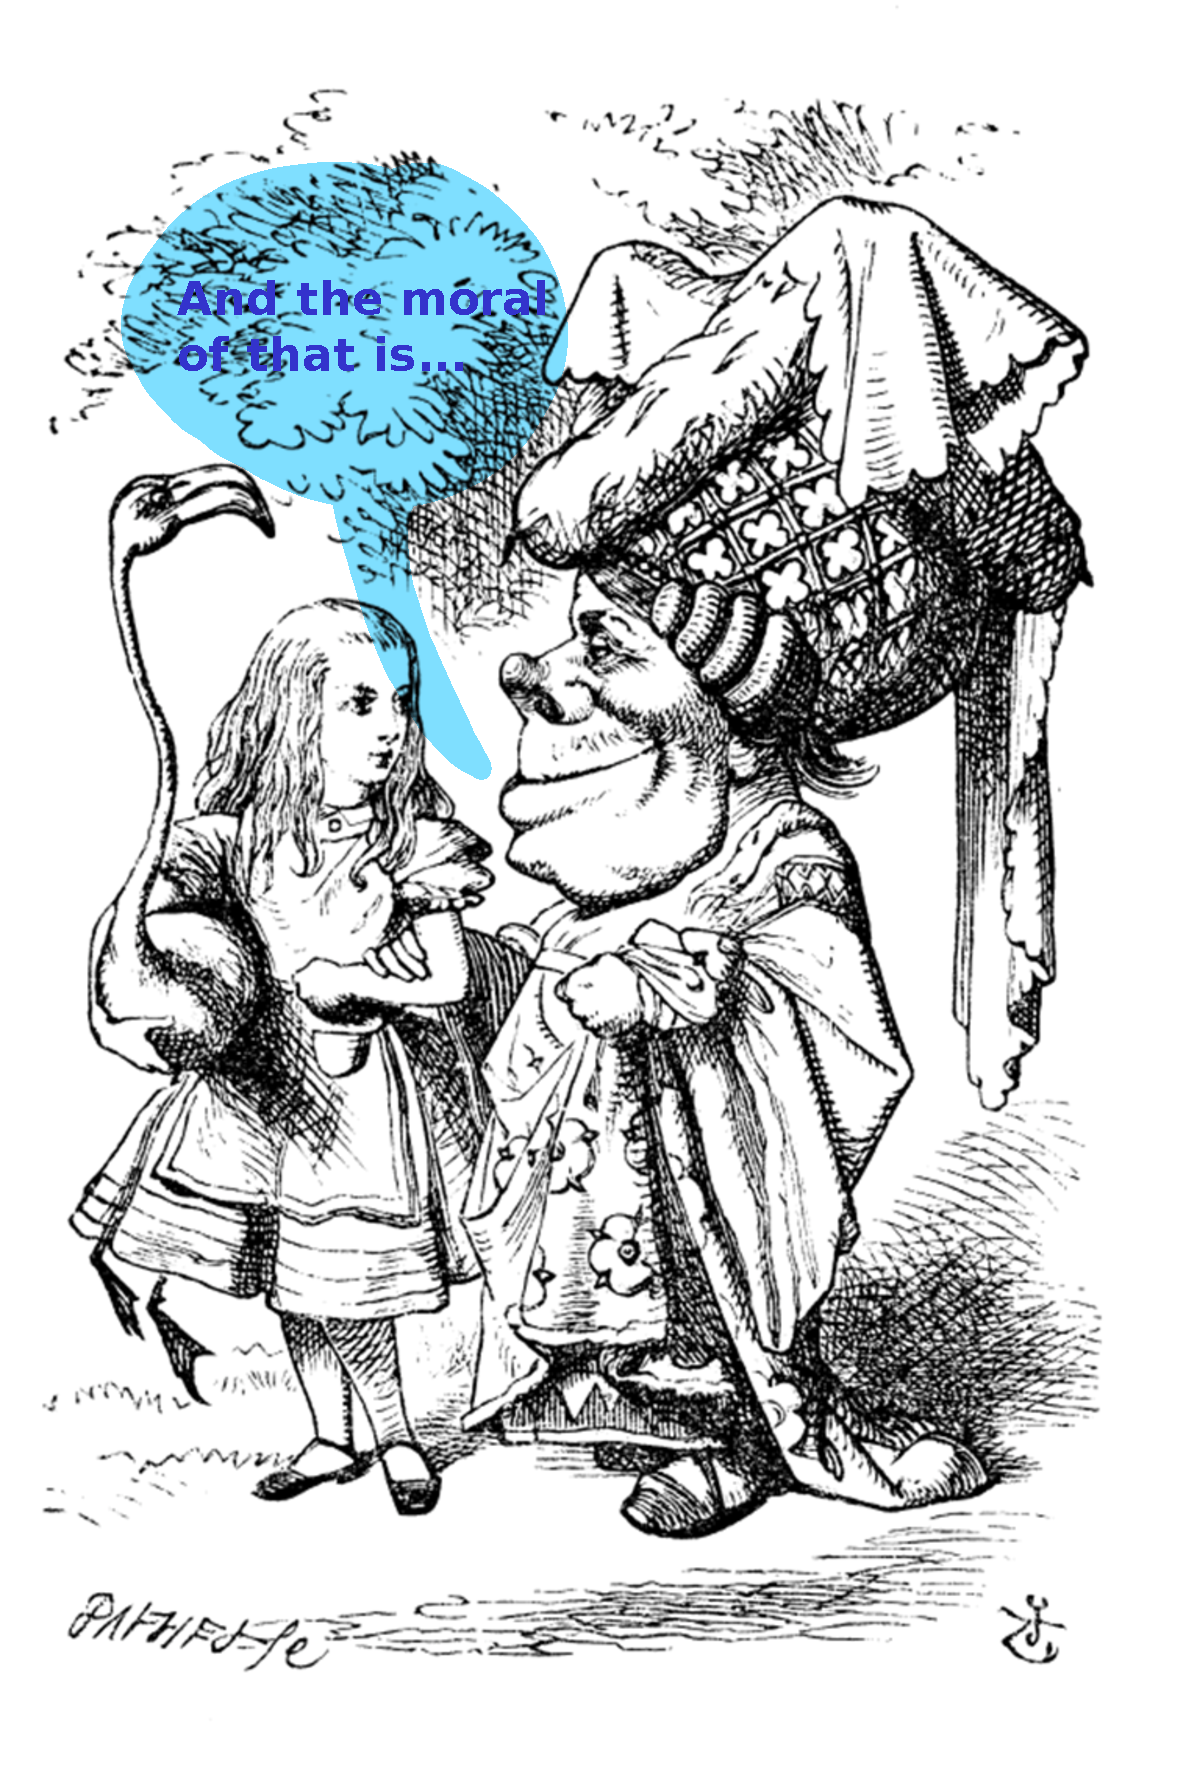
\includegraphics[width=\linewidth]{part2/Figures/1-the-duchess-moral}}
%		\end{center}		
%	\end{minipage}
%	\pause
%	\begin{minipage}{0.59\linewidth}
%		\dots a $f$ process with \emph{uncertainty} \\
%		is \emph{not deterministic}:\\
%		\begin{tabular}{ccc}
%			\tikzfig{deterministic_l} 
%			& $\neq$
%			& \tikzfig{deterministic_r}
%			\\
%			run $f$ multiple times 
%			&& run $f$ once\\
%			with same input
%			&& and copy output
%		\end{tabular}
%	\end{minipage}
%\end{frame}

\begin{frame}{Determinism in $\FinStoch$}
	Recall: $p : I \to A := \{a, b, c\}$ is a distribution $\{p(a), p(b), p(c)\}$. 
	\begin{example}
		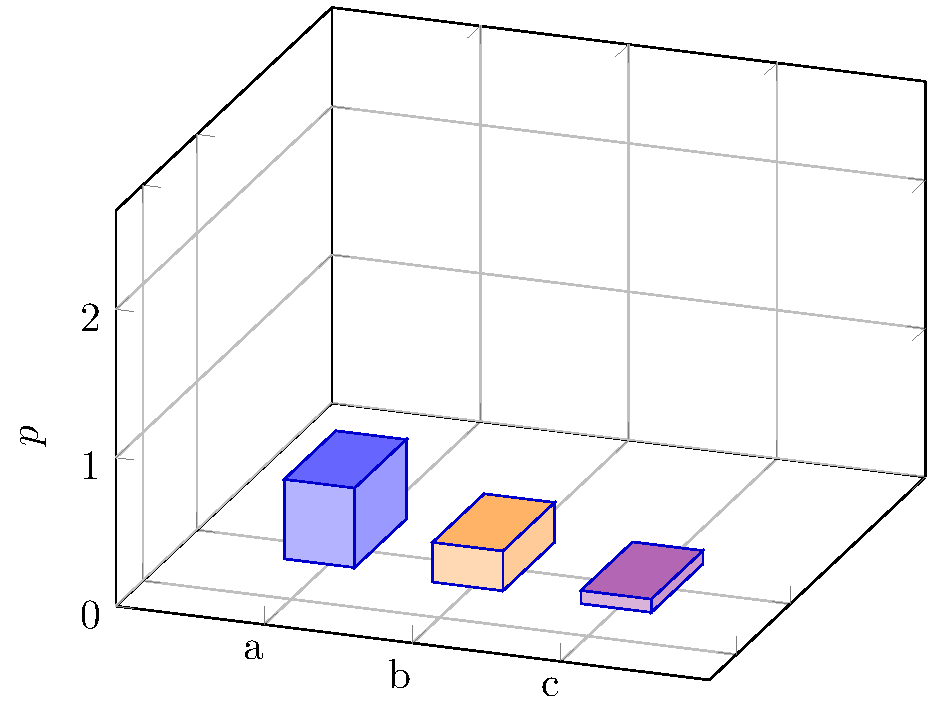
\includegraphics[scale=0.15]{part2/BarCharts/single_non-det}
		\pause is \emph{not} deterministic:
		\\ \pause
		\[ 
		\tikzfig{deterministic_I_l}
		= 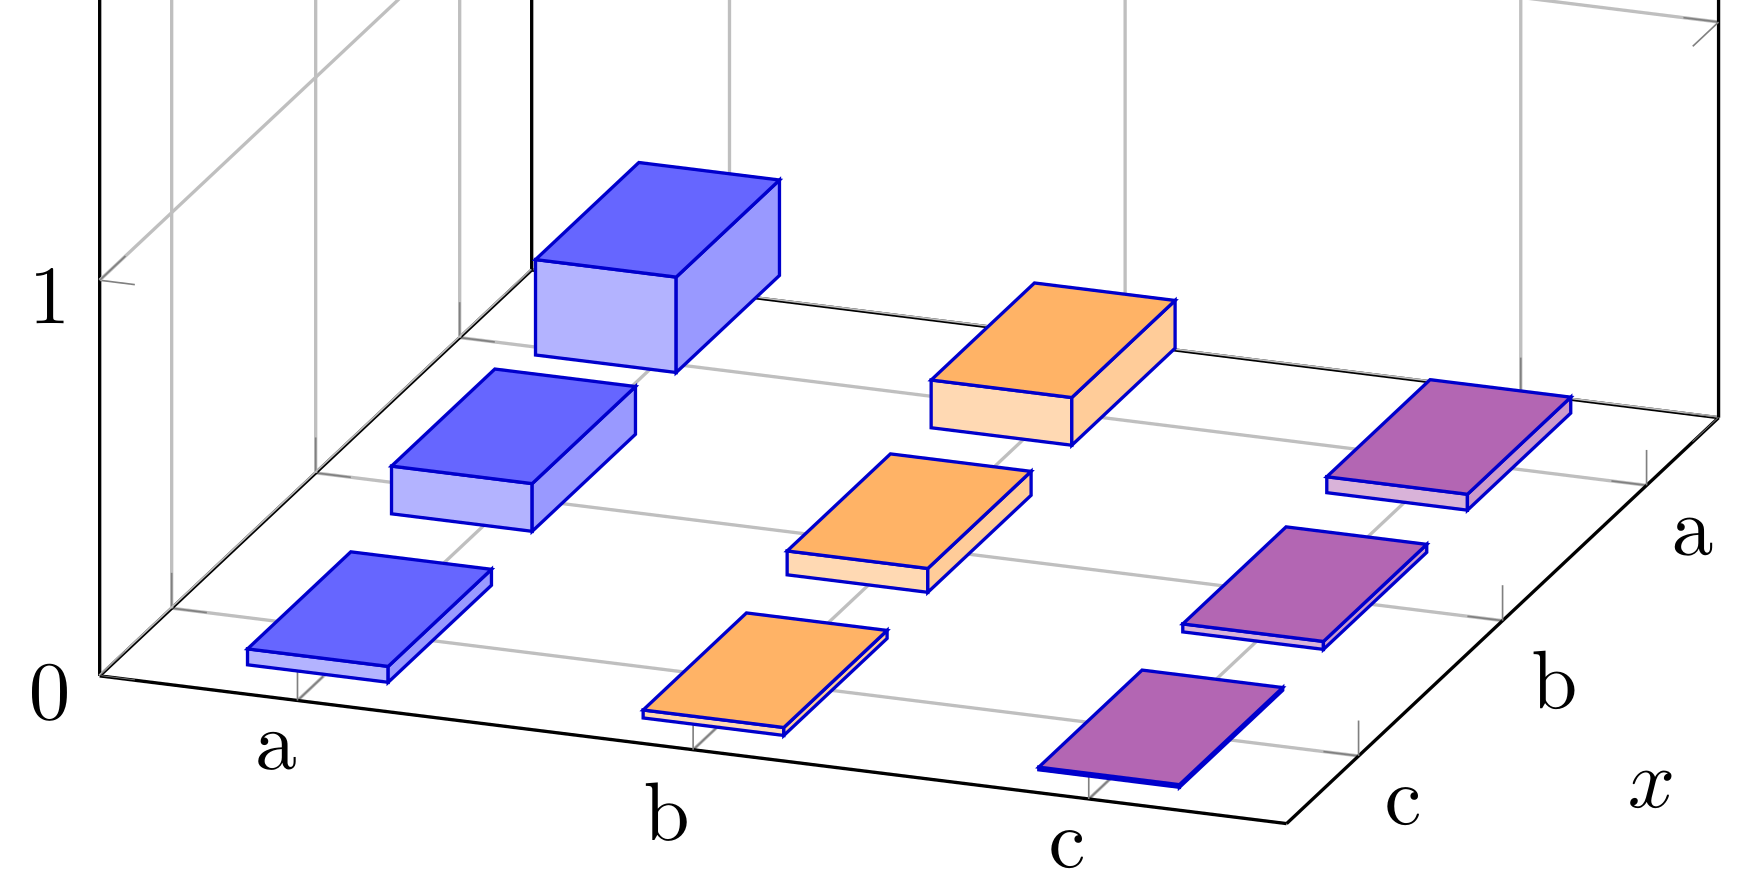
\includegraphics[scale=0.15]{part2/BarCharts/product_dist}
		\pause
		\neq 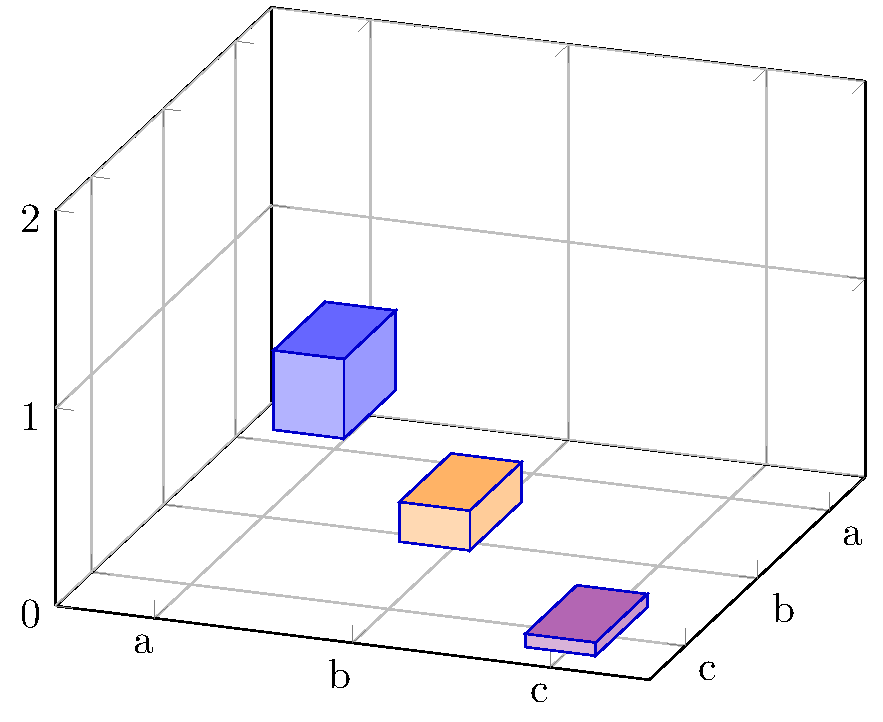
\includegraphics[scale=0.15]{part2/BarCharts/diagonal_dist}
		= \tikzfig{deterministic_I_r}
		\]
	\end{example}
\end{frame}

\begin{frame}{Determinism in $\FinStoch$}
	Recall: $p : I \to A := \{a, b, c\}$ is a distribution $\{p(a), p(b), p(c)\}$. 
	\begin{example}
		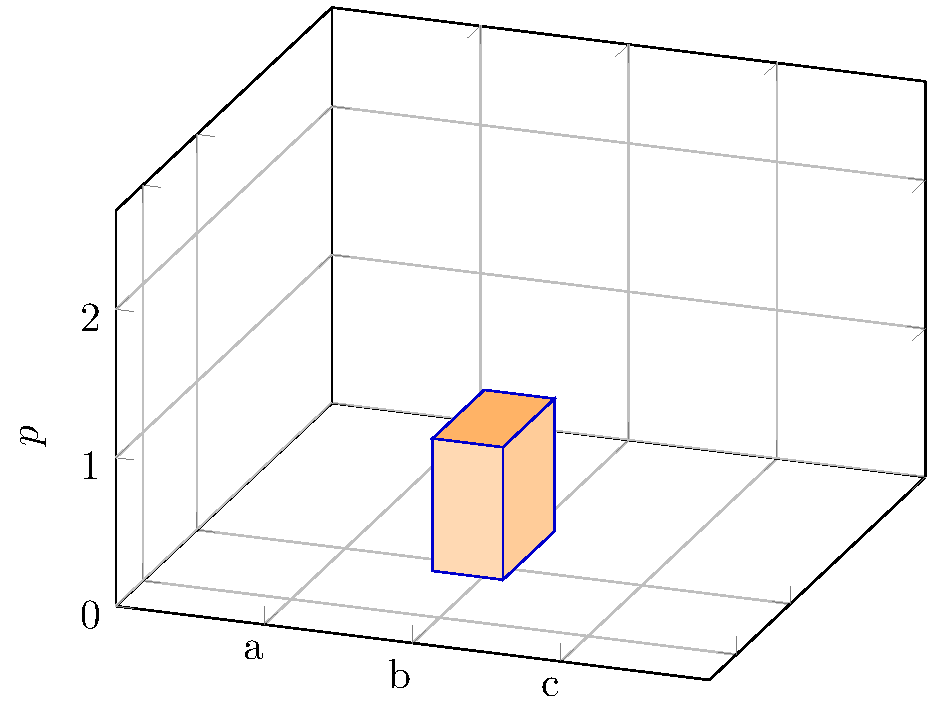
\includegraphics[scale=0.15]{part2/BarCharts/single_det}
		\pause is deterministic:
		\\
		\[ 
		\tikzfig{deterministic_I_l}
		= 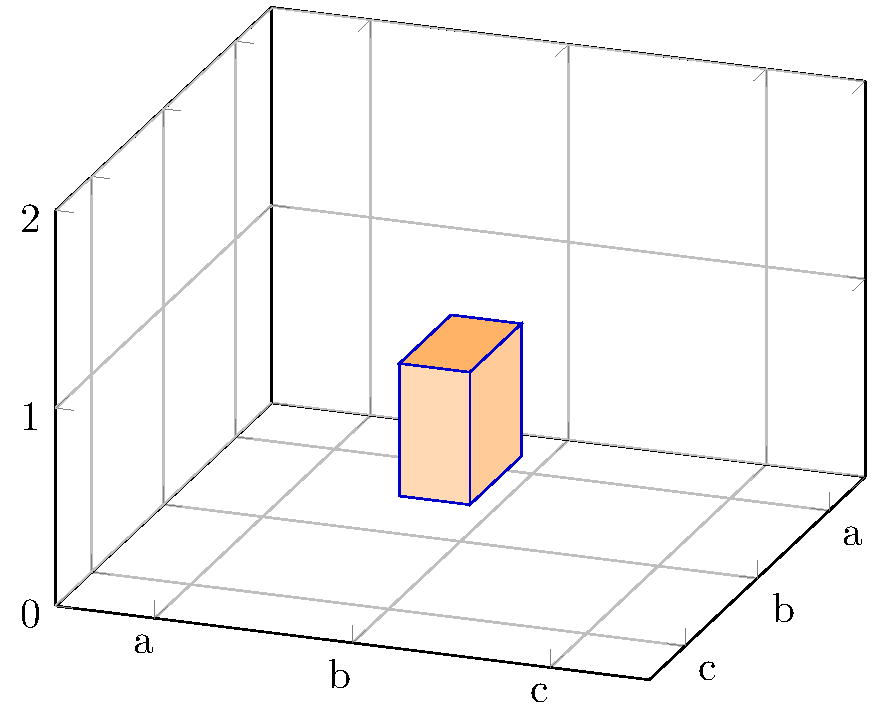
\includegraphics[scale=0.15]{part2/BarCharts/product_dist_det}
		= \tikzfig{deterministic_I_r}
		\]
	\end{example}
\end{frame}

\begin{frame}{Determinism in $\FinStoch$}
	Recall: $f : X \to Y$ has distributions $f_x$ on $Y$. 
%	\begin{minipage}{0.75\linewidth}
	\pause
	\begin{example}[\cite{Fritz_synthetic} Example 10.3.]
		\begin{tabular}{lll}
			$f$ is deterministic 
			& $\Leftrightarrow$ & all $f_x$ of form 
			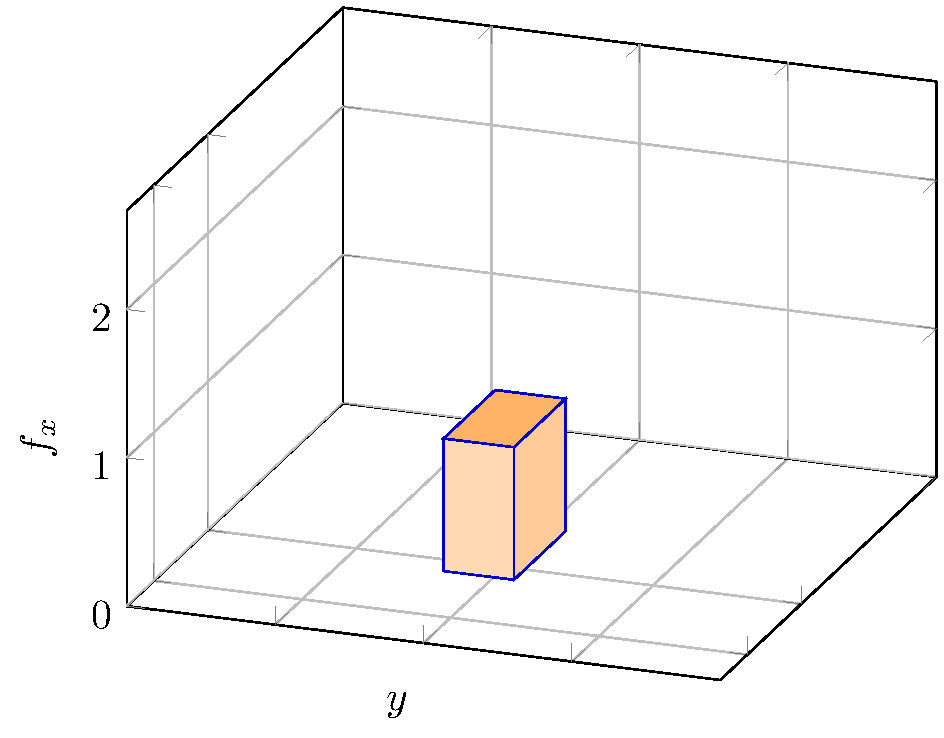
\includegraphics[scale=0.15]{part2/BarCharts/delta_det}
			\\
%			& $\Leftrightarrow$ & $f = \delta_{f'(\bullet)}$ for a $\cat{Set}$-function $f'$	\\
			& $\Leftrightarrow$ & $f$ corresponds to $\cat{Set}$-function
			\phantom{\qedhere}
		\end{tabular}
	%TODO "Observation"
	\end{example}
%	\end{minipage}
%	\begin{minipage}{0.24\linewidth}
%	\begin{center}
%		\makebox[\textwidth]{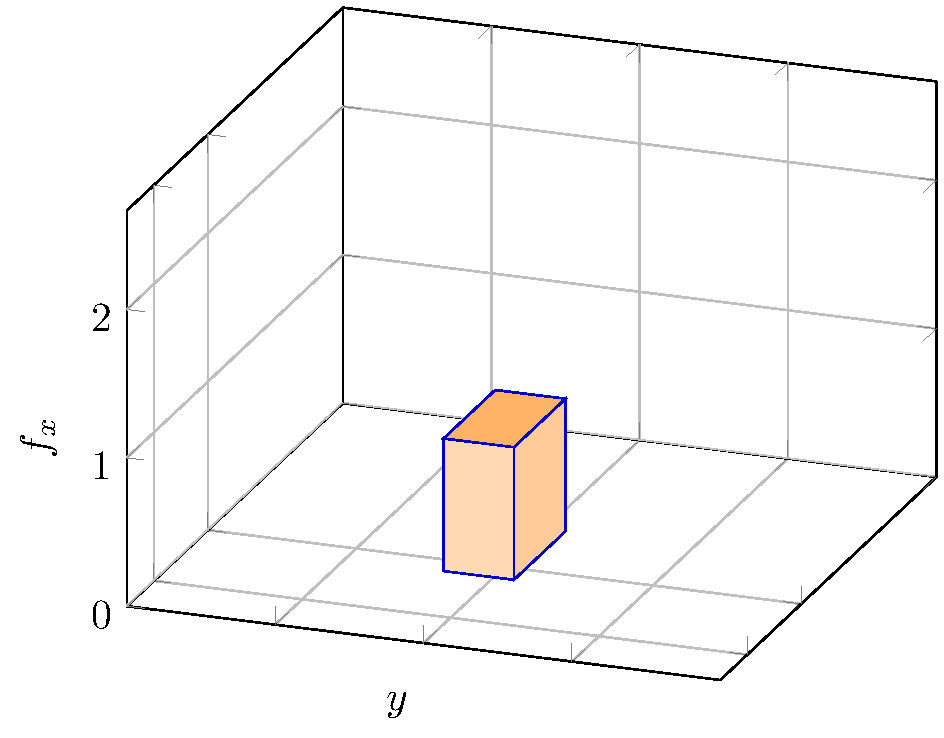
\includegraphics[width=\linewidth]{part2/BarCharts/delta_det}}
%	\end{center}		
%	\end{minipage}
%	\pause
%	\begin{lemma}
%		\[
%		\{ \text{Deterministic morphisms in $\FinStoch$} \}
%		\xleftrightarrow{1:1}
%		\cat{FinSet}
%		\]
%	\end{lemma}
%	\pause
%	Observation: $\cat{Set}$ is cartesian monoidal
\end{frame}

\begin{frame}{Determinism and Products}
	\begin{lemma}[\cite{Fritz_synthetic} Lemma 10.12, Remark 10.13.]
	For Markov category $\cC$ 
	\begin{itemize}
		\item deterministic morphisms form Markov subcategory $\cC_{\text{det}} \subset \cC$;
		\pause
		\item $\cC_{\text{det}}$ is cartesian monoidal (i.e. $\otimes$ is product functor).
%		\pause
%		\item If $\cC$ is cartesian monoidal, then all morphisms in $\cC$ are deterministic.
	\end{itemize}
	\end{lemma}
	\pause
	\begin{example}
		\[ 
		\FinStoch \supset \FinStoch_{\det} \cong \cat{FinSet}
		\]
	\end{example}
\end{frame}

\begin{frame}{Products and Determinism}
	\begin{lemma}[\cite{Fritz_synthetic} Remark 2.4.]
		For $\cC$ cartesian monoidal (i.e. $\otimes$ is product functor)
		\begin{itemize}
			\item $\cC$ is Markov;	% in a unique way!
			\item all morphisms are deterministic.
		\end{itemize}
		%		Cartesian monoidal categories are Markov categories (without uncertainty).
	\end{lemma}
	\pause
	\begin{example}[Markov categories without uncertainty]
		%\dots this includes
		$\cat{Set}$, $\cat{FinSet}$, $\cat{Top}$, \dots% $\cat{Top}$.
	\end{example}
\end{frame}

\begin{frame}{Probability Monads}
	\begin{minipage}{0.4\linewidth}
		\begin{center}
			\makebox[\textwidth]{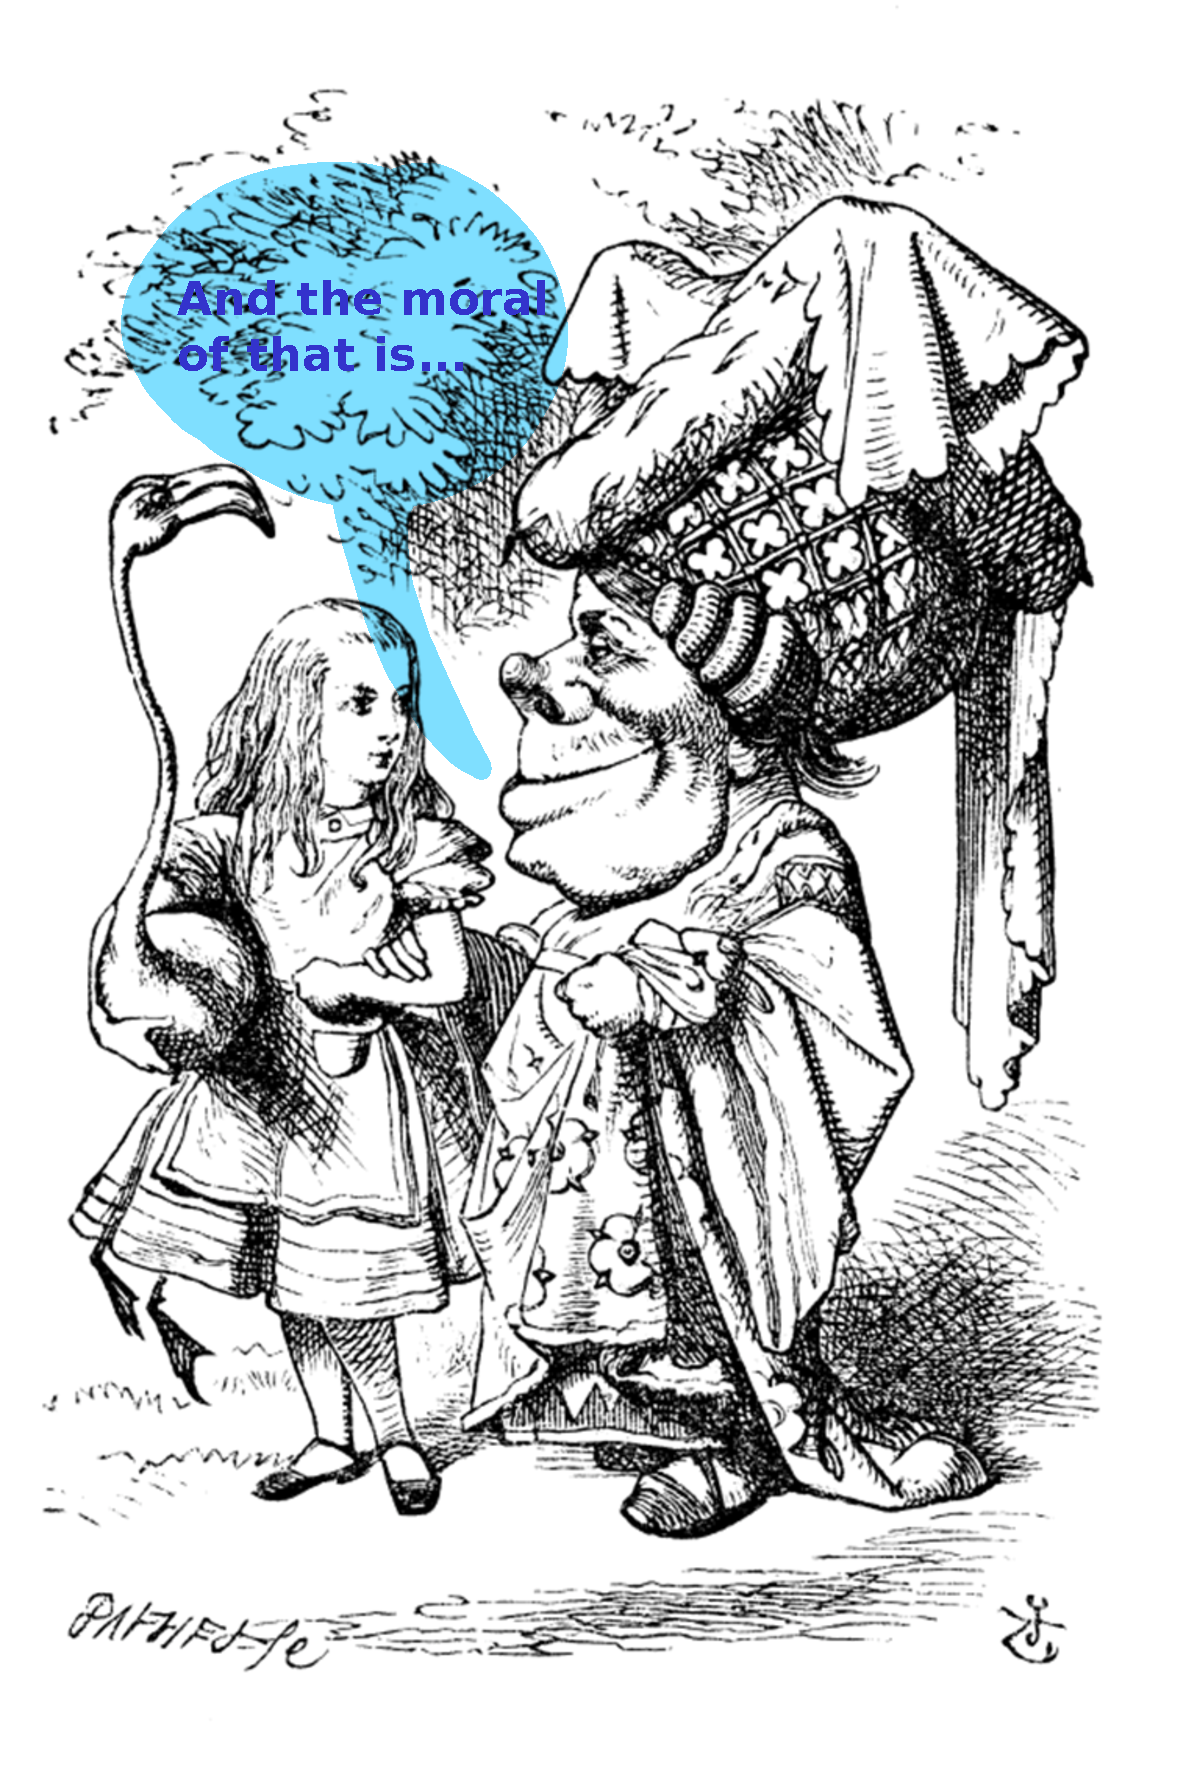
\includegraphics[width=\linewidth]{part2/Figures/1-the-duchess-moral}}
		\end{center}		
	\end{minipage}
%	\pause
	\begin{minipage}{0.59\linewidth}
		\centering
		Determinism $\leftrightsquigarrow$ Products	
	\end{minipage}
\end{frame}

\subsection{Probability Monads Introduce Uncertainty}

\begin{frame}{Probability Monads}
	\pause[2]
%	\emph{probability monads}
	\dots
	introduce uncertainty to cartesian Markov categories	
	\pause[1]
	\begin{example}[Deterministic Markov categories]
		%\dots this includes
		$\cat{Set}$, $\cat{FinSet}$, $\cat{Meas}$, $\cat{BorelMeas}$, \dots
		% $\cat{Top}$.
	\end{example}
%TODO Top, Vect, Man?

\end{frame}

\begin{frame}{Probability Monads}
	\begin{example}[Powerset Monad]
	\begin{center}
%		$\cat{Set}$ is cartesian monoidal $\Rightarrow$ morphisms are deterministic
		$\cat{Set}$ is deterministic
		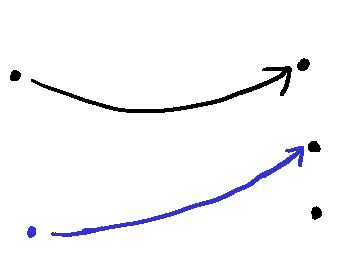
\includegraphics[scale=0.4]{part2/Figures/morphisms_set}
		\\ \pause 
			\rotatebox{-90}{$\rightsquigarrow$}\\
			(slightly adjusted) powerset monad 
			$2^{\circ} : \cat{Set} \to \cat{Set}$\\
			\pause
			\rotatebox[origin=c]{-90}{$\rightsquigarrow$}
			\\
		Kleisli category $\cat{Poss} := \cat{Set}_{2^{\circ}}$ %with morphisms 		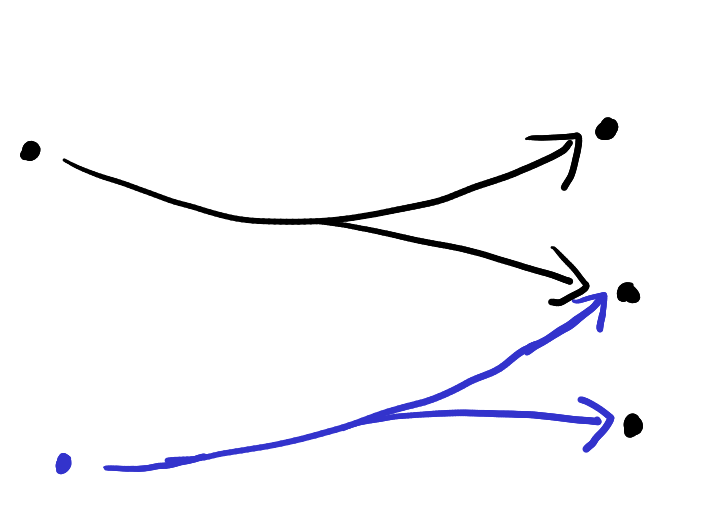
\includegraphics[scale=0.4]{part2/Figures/morphisms_poss} 
%			\begin{equation*}
%			\begin{split}
%			f : X &\to 2^Y	
%			\quad \text{i.e.~}
%			f(x) \subseteq Y
%			\end{split}
%			\end{equation*}
		describes \emph{possibility}
		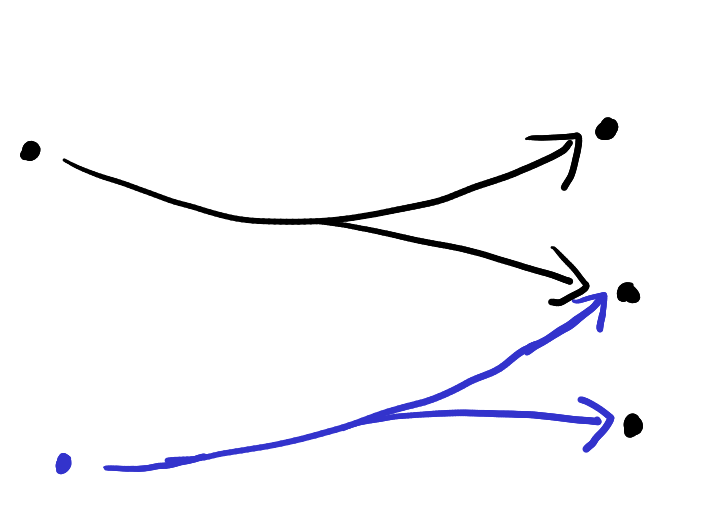
\includegraphics[scale=0.4]{part2/Figures/morphisms_poss} 
	\end{center}
	\end{example}
\end{frame}

\begin{frame}{Probability Monads}
	\begin{theorem}[\cite{Fritz_representable}, Proposition 3.1.]
%		{\pause[1]
		For $\cC$ cartesian monoidal, monad $T: \cC \to \cC$ 
		\begin{itemize}
			\item compatible with $I$	% affine: I \cong T(I)
%			{\pause[2] 
			{\color{gray}($\rightsquigarrow$ powerset monad was adjusted)}
%			}
			\item compatible with $\otimes$ and symmetry
										% symmetric monoidal monad:
										% monoidal functor compatibel with 
										% - unit of T
										% - multiplication of T
										% - symmetric braiding 
		\end{itemize}
		Kleisli category $\cC_T$ is Markov.
%	}
	\end{theorem}
\end{frame}

%\begin{frame}{Probability Monads}
%	\begin{example}[Giry Monad]
%		
%	Cartesian monoidal category $\cat{Meas}$ with
%	\begin{itemize}
%			\item objects: \enquote{sets with observable subsets} 
%%			& \multirow{2}{}{is cartesian monoidal}
%%			\\
%			\item morphisms: $\cat{Set}$-functions compatible with observability
%	\end{itemize}
%	\begin{center}
%		\rotatebox{-90}{$\rightsquigarrow$}\\
%%		\begin{tabular}{rcl}
%%			Giry monad $G : \cat{Meas}$
%%			&	$\to$ 
%%			&		$\cat{Meas}$\\
%%			$X$
%%			&	$\mapsto$ 
%%			&		\{probability distributions on $X$\}
%%		\end{tabular}
%		Giry monad $G : \cat{Meas} \to \cat{Meas}$
%		\\ \pause
%		\rotatebox[origin=c]{-90}{$\rightsquigarrow$}
%		\\
%		Markov cat. $\cat{Meas}_G =: \cat{Stoch}$ describing probabilistic transitions.
%	\end{center}	
%	\end{example}
%\end{frame}

\begin{frame}{Probability Monads}
	\begin{example}
	% https://q.uiver.app/#q=WzAsMTAsWzIsMF0sWzAsMF0sWzQsMCwiXFxjYXR7U2V0fSJdLFs0LDIsIlxcY2F0e1Bvc3N9Il0sWzYsMCwiXFxjYXR7RmluU2V0fSJdLFs2LDIsIlxcY2F0e0ZpblBvc3N9Il0sWzgsMCwiXFxjYXR7TWVhc30iXSxbOCwyLCJcXGNhdHtTdG9jaH0iXSxbMTAsMCwiXFxjYXR7Qm9yZWxNZWFzfSJdLFsxMCwyLCJcXGNhdHtCb3JlbFN0b2NofSJdLFsyLDMsIjJee1xcY2lyY30iLDEseyJzdHlsZSI6eyJib2R5Ijp7Im5hbWUiOiJzcXVpZ2dseSJ9fX1dLFs0LDUsIjJee1xcY2lyY30iLDFdLFs2LDcsIkciLDEseyJzdHlsZSI6eyJib2R5Ijp7Im5hbWUiOiJzcXVpZ2dseSJ9fX1dLFs4LDksIkciLDEseyJzdHlsZSI6eyJib2R5Ijp7Im5hbWUiOiJzcXVpZ2dseSJ9fX1dXQ==
	\[\begin{tikzcd}[ampersand replacement=\&]
	{\cat{Set}} \&\& {\cat{FinSet}} \&\& {\cat{Meas}} \&\& {\cat{BorelMeas}} \\
	\\
	{\cat{Poss}} \&\& {\cat{FinPoss}} \&\& {\cat{Stoch}} \&\& {\cat{BorelStoch}}
	\arrow["{2^{\circ}}"{description}, squiggly, from=1-1, to=3-1]
	\arrow["{2^{\circ}}"{description}, squiggly, from=1-3, to=3-3]
	\arrow["\text{Giry monad}"{description}, squiggly, from=1-5, to=3-5]
	\arrow["\text{Giry monad}"{description}, squiggly, from=1-7, to=3-7]
	\end{tikzcd}\]
	\end{example}
	%
\end{frame}


\begin{frame}{Probability Monads}
	\begin{minipage}{0.4\linewidth}
		\begin{center}
			\makebox[\textwidth]{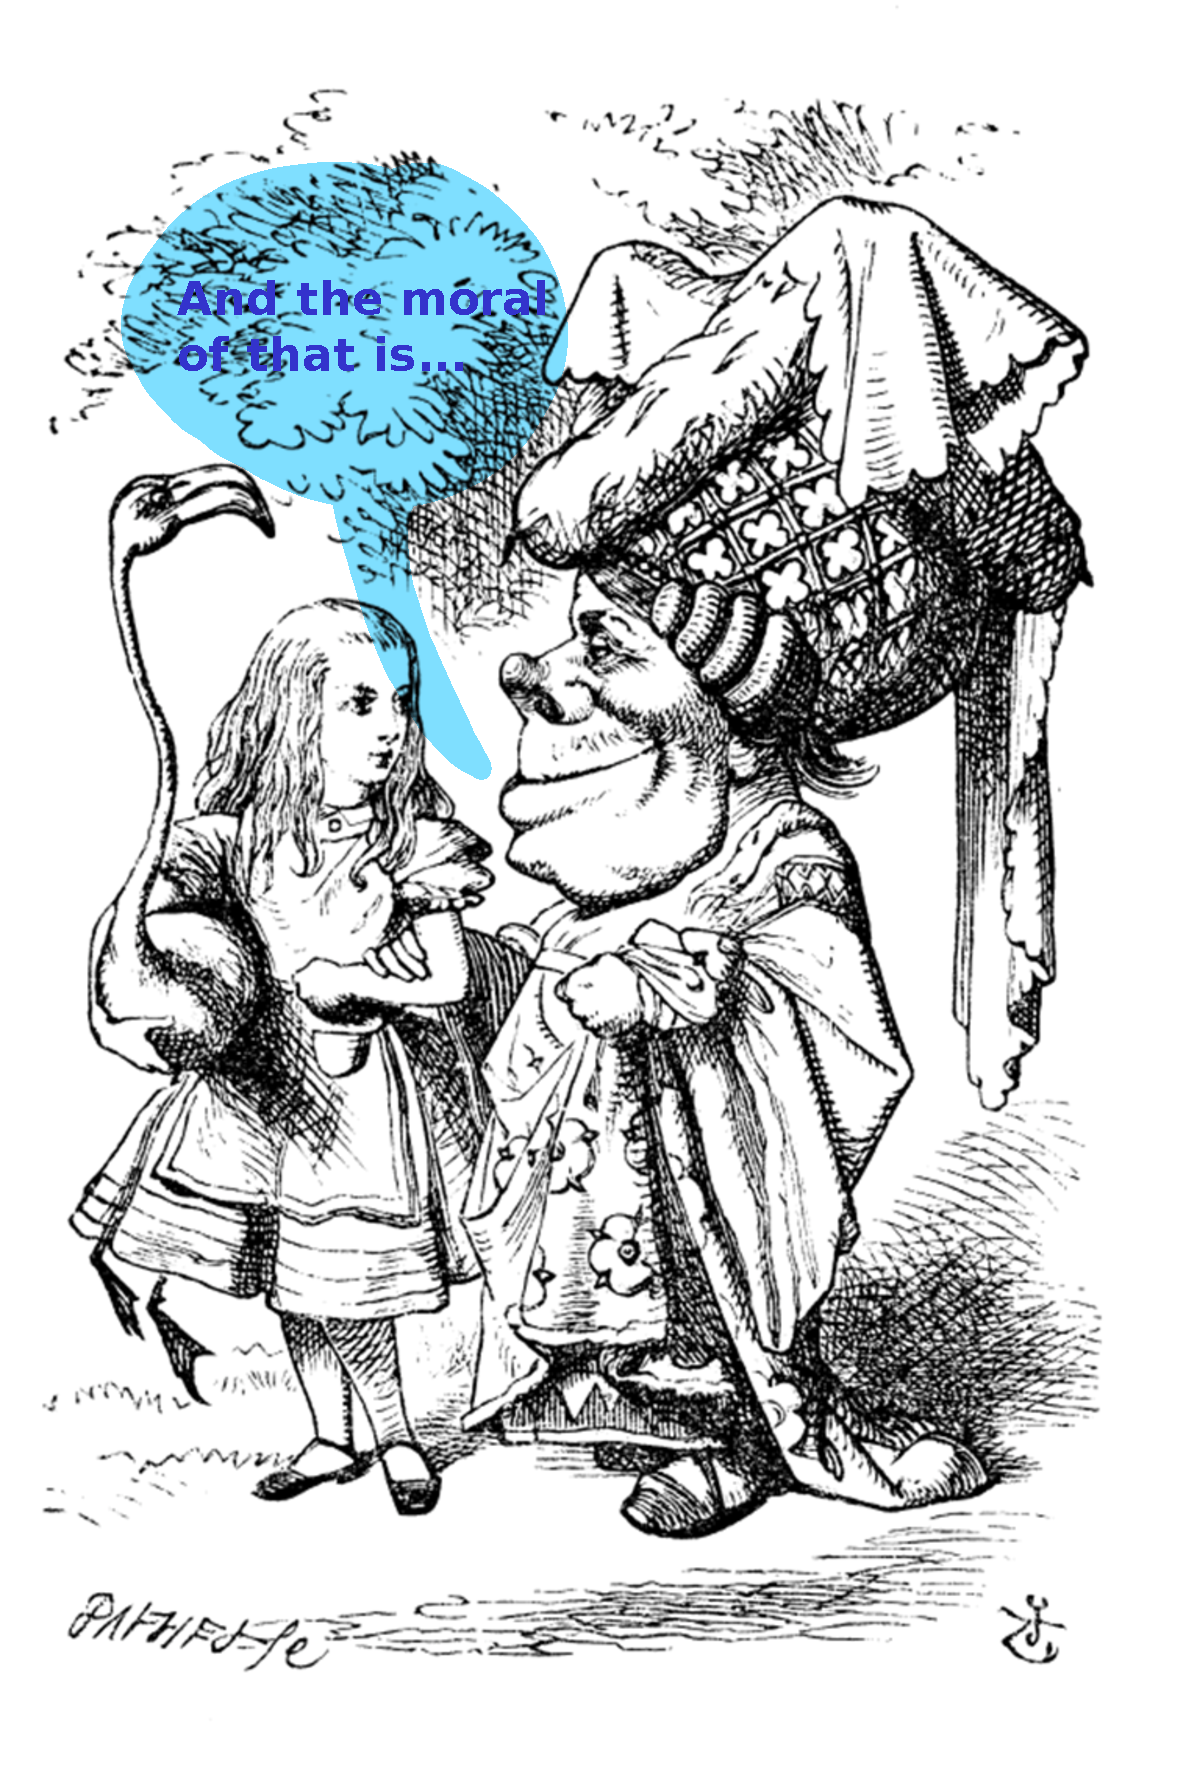
\includegraphics[width=\linewidth]{part2/Figures/1-the-duchess-moral}}
		\end{center}		
	\end{minipage}
	\pause
	\begin{minipage}{0.59\linewidth}
		Uncertainty is incorporated in \emph{morphisms}!
	\end{minipage}
\end{frame}

\subsection{Representable Markov Categories}
\begin{frame}{Representability}
	%TODO delete this?
	Monads introduce uncertainty, i.e.\,\emph{non-deterministic} morphisms:
	\begin{example}
		% https://q.uiver.app/#q=WzAsMTAsWzIsMF0sWzAsMF0sWzQsMCwiXFxjYXR7U2V0fSJdLFs0LDIsIlxcY2F0e1Bvc3N9Il0sWzYsMCwiXFxjYXR7RmluU2V0fSJdLFs2LDIsIlxcY2F0e0ZpblBvc3N9Il0sWzgsMCwiXFxjYXR7TWVhc30iXSxbOCwyLCJcXGNhdHtTdG9jaH0iXSxbMTAsMCwiXFxjYXR7Qm9yZWxNZWFzfSJdLFsxMCwyLCJcXGNhdHtCb3JlbFN0b2NofSJdLFsyLDMsIjJee1xcY2lyY30iLDEseyJzdHlsZSI6eyJib2R5Ijp7Im5hbWUiOiJzcXVpZ2dseSJ9fX1dLFs0LDUsIjJee1xcY2lyY30iLDFdLFs2LDcsIkciLDEseyJzdHlsZSI6eyJib2R5Ijp7Im5hbWUiOiJzcXVpZ2dseSJ9fX1dLFs4LDksIkciLDEseyJzdHlsZSI6eyJib2R5Ijp7Im5hbWUiOiJzcXVpZ2dseSJ9fX1dXQ==
		\[\begin{tikzcd}[ampersand replacement=\&]
		{\cat{Set}} \&\& {\cat{FinSet}} \&\& {\cat{Meas}} \&\& {\cat{BorelMeas}} \\
		\\
		{\cat{Poss}} \&\& {\cat{FinPoss}} \&\& {\cat{Stoch}} \&\& {\cat{BorelStoch}}
		\arrow["{2^{\circ}}"{description}, squiggly, from=1-1, to=3-1]
		\arrow["{2^{\circ}}"{description}, squiggly, from=1-3, to=3-3]
		\arrow["\text{Giry monad}"{description}, squiggly, from=1-5, to=3-5]
		\arrow["\text{Giry monad}"{description}, squiggly, from=1-7, to=3-7]
		\end{tikzcd}\]
	\end{example}
	\begin{center}
	Question: 
	Do they also introduce \emph{deterministic} morphisms?
	\end{center}
\end{frame}

\begin{frame}{Representability}
%	\begin{minipage}{0.45\linewidth}
		\begin{definition}[Representability]
			Markov cat. $\cC$ is \emph{representible}, if
			\begin{itemize}
				\item $\cC \cong \cat{D}_{T}$ for monad $T : \cat{D} \to \cat{D}$
				\item $\cat{D} \cong \cC_{\det}$.
			\end{itemize}
		\end{definition}
		%	\hfill
%	\end{minipage}
%	~~
	\pause
	\begin{minipage}{0.5\linewidth}
		%	\begin{example}
		%		($\cat{Fin}$)$\cat{Stoch}$ \emph{not} representable.\\
		%			\pause
		%			\item 
		%			$\cat{BorelStoch}$, ($\cat{Fin}$)$\cat{Poss}$ are.
		%		\end{itemize}
		%	\end{example}
		\begin{example}
			$\cat{BorelStoch}$, ($\cat{Fin}$)$\cat{Poss}$ representable.
		\end{example}
	\end{minipage}
	~~ \pause 
	\begin{minipage}{0.45\linewidth}
		\begin{example}
			($\cat{Fin}$)$\cat{Stoch}$ \emph{not} representable.
		\end{example}
		%	\hfil
	\end{minipage}
	%TODO Gauss?
\end{frame}